\documentclass[10pt,twocolumn,letterpaper]{article}

\usepackage{cvpr}
\usepackage{times}
\usepackage{epsfig}
\usepackage{graphicx}
\usepackage{amsmath}
\usepackage{amssymb}

% Include other packages here, before hyperref.

% If you comment hyperref and then uncomment it, you should delete
% egpaper.aux before re-running latex.  (Or just hit 'q' on the first latex
% run, let it finish, and you should be clear).
\usepackage[breaklinks=true,bookmarks=false]{hyperref}

\cvprfinalcopy % *** Uncomment this line for the final submission

\def\cvprPaperID{****} % *** Enter the CVPR Paper ID here
\def\httilde{\mbox{\tt\raisebox{-.5ex}{\symbol{126}}}}

% Pages are numbered in submission mode, and unnumbered in camera-ready
%\ifcvprfinal\pagestyle{empty}\fi
\setcounter{page}{4321}
\begin{document}

%%%%%%%%% TITLE
\title{\LaTeX\ A }

\author{Shan Zhou \\
Facebook \\
\\
{\tt\small shanzhou@stanford.edu}
% For a paper whose authors are all at the same institution,
% omit the following lines up until the closing ``}''.
% Additional authors and addresses can be added with ``\and'',
% just like the second author.
% To save space, use either the email address or home page, not both
\and
Timothy Daley \\
Stanford University \\
Departments of Statistics and Bioengineering \\
{\tt\small tdaley@stanford.edu}
}

\maketitle
%\thispagestyle{empty}

%%%%%%%%% ABSTRACT
\begin{abstract}
TODO   
\end{abstract}

%%%%%%%%% BODY TEXT
\section{Introduction}

Predicting tumor growth rate is a first step in determining treatment options for cancer patients.  Fast growing tumors necessarily require more aggressive treatment.  It would be beneficial if patients could avoid aggressive treatments when possible.  

Alexandra Sockell of the Fordyce and Curtis labs in the Bioengineering and Genetics departments, respectively, of Stanford University has developed a microfluidic device to isolate single cells of a tumor and allow them to grow into organoids  within the microwell.  Organoids are three dimensional stem cell-like cultures that organize into a "mini-organ"~\cite{rios2018imaging}, and can be used to study cancer in a more natural environment than traditional cell lines~\cite{drost2018organoids}.
The objective of her research is to study the mechanisms of tumor growth by subjecting a large number of  individual cells to a wide range of treatments and conditions and track their condition by imaging.  She has taken 14 days of imaging over approximately 40 conditions.    For each day, there are approximate 200,000 well images across all conditions.  The number of cells per well is approximately Poisson, with most of the wells not containing any cells, 25\% have one cell, and smaller portion have more than 1.  We believe that the large number of images should provide a sufficient amount of data and information content to apply deep convolution neural network approach.  Our hypothesis is that the state of the cells in the early days should be related to their final state.  Therefore our objective to determine whether the early stages of the organoid can predict the growth rate and final state of the organoid.    

Previous approaches for high-throughput analysis of organoid imaging data did not look at single-cell microwell level data.  Instead they typically relied upon a large number of cells to quantify cell proliferation or death \cite{jabs2017screening},  used cell counting assays to calculate growth \cite{sebrell2018live}, or used single cell tracking to calculate cell motility \cite{geum2016epidermal}.  To our knowledge, no deep learning approaches have been proposed to analyse organoid imaging data, despite the large success in deep learning to analysing imaging data across a broad spectrum of applications.

\section{Data}

To achieve the goal of predicting tumor growth, we took the objective as predicting the final size of the tumor after 13 days of growth.  The final size is calculated by image segmentation of the interior of the microwell (Fig\ref{workflow}).  We normalized the sizes to have variance equal to one.  However, we did not mean center the data because we believe a final size equal to zero has meaning.  A final size equal to zero corresponds to either empty wells or cells that died.  

\begin{figure}[b!]
\begin{center}
 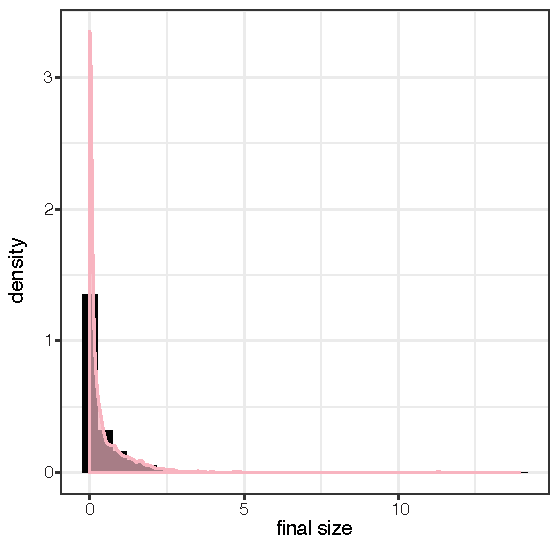
\includegraphics[width=0.8\linewidth]{figures/final_day_hyst2_area_density.pdf}
\end{center}
   \caption{Distribution of normalized final sizes.  There is a large peak at zero corresponding to empty wells or cells that died.}
\label{final_size_dist}
\end{figure}

For input we took the day 1 images.  We determined that the day 0 images are not suffcient to predict  All images are black and white, so we converted them to greyscale and normalized the pixels to have zero mean and unit variance.  Our resulting images are 193$\times$193 with a single channel.   An example input image is show in figure~\ref{workflow}.




\begin{figure*}[t!]
\begin{center}
 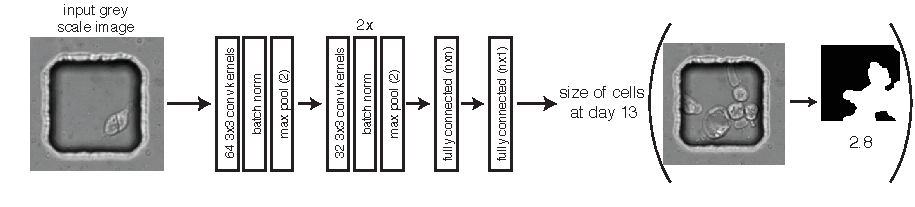
\includegraphics[width=0.8\linewidth]{figures/networkExampleImage.pdf}
\end{center}
   \caption{Example workflow of our algorithm.  The input is a 193$\times$193 greyscale image of the cell at day one.  We pass this through a convolutional neural network to predict the final size, normalized to have variance equal to 1.}
\label{workflow}
\end{figure*}

\section{Model}

To show the feasibility of a deep convolutional approach, we constructed two preliminary deep learning models. One consists of three convolutional layers, applying batch normalization and max pooling to each layer, followed by two fully connected layers. The other consist of four layers with three convolution layers and one fully connected layer. We tried different kernal size, batch size, optimizer and learning rate. The Adam Optimizer and learning rate 1e-4 produce best result for the preliminary models.
As an initial test we use one hundred randomly selected images as a training set and another one hundred randomly selected images as a validation set.  


\begin{figure*}[t!]
\begin{center}
 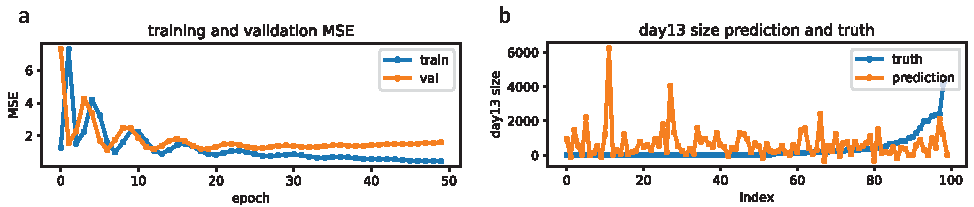
\includegraphics[width=0.8\linewidth]{figures/error_vs_epoch_and_validation_predictions_vs_observed.pdf}
\end{center}
   \caption{\textbf{a} The training error (blue) and validation error (orange) as a function of training epoch.  \textbf{b} Predicted final size and observed final size, with the index ordered by observed final size. }
\label{workflow}
\end{figure*}



\section{Preliminary Results}



{\small
\bibliographystyle{ieee}
\bibliography{bib}
}

\end{document}
